\chapter{Progettazione}

Nella fase di progettazione, si sono fatte alcune assunzioni sull'ambiente, sul drone e sulle altre entità coinvolte durante la fase di simulazione.
In particolare, tali assunzioni riguardano le caratteristiche principali dell'ambiente e delle entità in esso coinvolte.

\section{Progettazione dell'ambiente}

L'ambiente che viene preso in esame dipende dallo scenario considerato per la simulazione della missione.
Esso rappresenta un'area bidimensionale strutturata e limitata, in cui lo spazio ed il tempo risultano entrambi discretizzati.

Lo spazio è simulato attraverso una griglia di \textit{NxM} celle quadrate, dette \textit{patch}, di lato \textit{S}. 
Il tempo è discretizzato in una sequenza di intervalli temporali di durata \textit{T} detti \textit{tick} definiti come:
\begin{equation*}
    t_0 + T, t_0 + 2T, \dots, t_0 + NT
\end{equation*}

L'ambiente simulato contiene i seguenti elementi: 
\begin{itemize}
    \item \textit{Droni};
    \item \textit{Target};
    \item \textit{Ostacoli};
    \item \textit{Feromoni digitali};
\end{itemize}

La figura \ref{elementi_ambiente} mostra una rappresentazione semplificata dell'ambiente di simulazione con gli elementi sopra descritti.

Nell'ambiente, un singolo UAV è rappresentato da un disco con un punta di freccia interna. 
La punta indica la direzione del drone. 
Ostacoli e target, solitamente, coprono diverse celle.
In figura, ogni cella in cui è presente un ostacolo è nera, mentre ogni cella-target è colorata. 
Come abbiamo già precedentemente accennato, un target può assumere diversi stati: in questo caso un target \textit{not found} è rappresentato da una cella rossa, un target \textit{found} da una cella verde e con una cella gialla, infine, un target \textit{executed}.
L'intensità del colore di bersaglio, quando applicabile (ad esempio, fuoco, gas, ecc.), rappresenta la quantità/presenza del target. 
Infine, una traccia feromonica è indicata da un gruppo di cellule grigie, dove la scala di grigio varia in base all'intensità dei feromoni.

\begin{figure}[H] 
    \captionsetup{justification=centering, margin=2cm, font=footnotesize}
    \begin{center}
    \makebox[\textwidth]{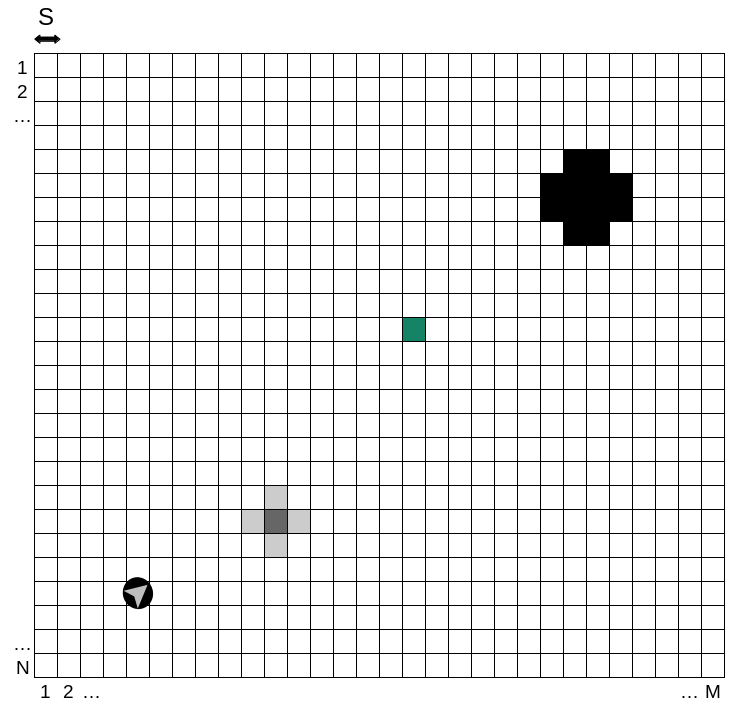
\includegraphics[width=0.4\paperwidth]{img/elementi_ambiente.png}}
    \end{center}
    \caption[short]{Definizione dell'ambiente simulato: (da sinistra a destra) drone, feromone, target ed ostacolo.}
    \label{elementi_ambiente}
\end{figure}

Si assumano, per semplicità i seguenti valori:
\begin{itemize}
    \item S = 1 metro;
    \item T = 1 secondo; 
\end{itemize}

I valori sopra riportati, naturalmente, possono variare in base alla missione ed allo scenario in cui essa si svolge.
In questo caso, l'assunzione è necessaria per una conversione immediata da metri a numero di patch e da secondi a tick.

Supponendo di avere una patch di lato \textit{S} diverso da un metro, può essere sfruttata la seguente formula di conversione, per determinare il numero di patch a cui corrisponde un metro:

\begin{equation}
    \label{m_patches}
    1 \; m = \frac{1}{S} \; patches
\end{equation}

Allo stesso modo, si può determinare a quanti tick corrisponde un secondo:

\begin{equation}
    \label{sec_ticks}
    1 \; s = \frac{1}{T} \; ticks
\end{equation}

Dalle relazioni \ref{m_patches} e \ref{sec_ticks} è possibile determinare la formula di conversione da \textit{m/s} a \textit{patches/tick}:

\begin{equation*}
    1 \; m/s = (\frac{1}{S})(\frac{1}{T}) \; patches/tick 
\end{equation*}

Ad ogni tick, il drone effettua rilevamenti di ostacoli, target e feromoni vicini alla sua posizione ed esegue regole comportamentali precise.
Lo sciame di droni si muove separatamente, organizzato in diversi flock.

Il blocco fondamentale dello spazio discretizzato simulato è rappresentato dalla cella.
Ogni cella (denominata anche patch) ha delle coordinate \textit{x-y} nello spazio bidimensionale e può contenere un target o un ostacolo.
Una caratteristica fondamentale del simulatore è la possibilità di prenotare una patch: tale strategia, infatti, è pensata nel caso in cui è previsto un meccanismo di \textit{collision avoidance}, come nel caso dell'algoritmo SCIADRO.

Per illustrare la struttura di un oggetto \textit{patch}, consideriamo la cella come una classe.
Nella figura \ref{classe_patch} è possibile osservare tale struttura.

\begin{figure}[H] 
    \captionsetup{justification=centering, margin=2cm, font=footnotesize}
    \begin{center}
    \makebox[\textwidth]{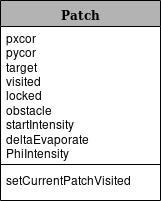
\includegraphics[width=0.2\paperwidth]{img/classe_patch.png}}
    \end{center}
    \caption[short]{Struttura della classe Patch.}
    \label{classe_patch}
\end{figure}

\section{Elemento ostacolo}

Un ostacolo è un elemento che ostruisce il passaggio di un UAV. 
Esso ha una posizione statica e occupa una cella all’interno dell’ambiente di esplorazione. 
L’ostacolo non può essere attraversato dal drone e rappresenta la base per modellare diversi tipi di strutture come, ad esempio, alberi, costruzioni, ecc.

\section {Elemento target}

Un target è un elemento collocato, all'istante \textit{t}, in una determinata posizione dell’ambiente di simulazione sconosciuta ai droni. 
La struttura di un target dipende da cosa si vuole modellare, in accordo con il task della missione:

\begin{itemize}
    \item \textit{Rilevamento di sostanze}, come un gas o un liquido tossico: in questo caso gli elementi sono modellati attraverso una distribuzione gaussiana di target, con media in corrispondenza della sorgente;
    \item \textit{Identificazione di oggetti}, come ad esempio mine anti-uomo: in questo caso il target è modellato come una singola cella;
    \item \dots
\end{itemize}

Lo stato di un target è identificato dalla variabile \textbf{target.state}, che può assumere i seguenti valori:

\begin{itemize}
    \item \textit{Found};
    \item \textit{Not found};
    \item \textit{Executed}.
\end{itemize}

\begin{figure}[H] 
    \captionsetup{justification=centering, margin=2cm, font=footnotesize}
    \begin{center}
    \makebox[\textwidth]{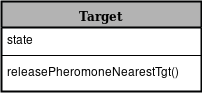
\includegraphics[width=0.2\paperwidth]{img/classe_target.png}}
    \end{center}
    \caption[short]{Struttura della classe Target.}
    \label{classe_target}
\end{figure}

\section {Elemento UAV}

L'UAV è l'elemento in grado di muoversi in modo continuo all’interno dello spazio bidimensionale di ricerca con l’obiettivo principale di scoprire nuovi target. 
Inoltre, il drone deve evitare di scontrarsi con gli ostacoli o con altri droni e, insieme a loro, deve coordinarsi e completare il processo di scoperta dei target entro il tempo di autonomia, usando meccanismi di comunicazione diretta o indiretta, in base all’algoritmo integrato nel simulatore. 

Gli scontri e le collisioni con altri droni e con gli ostacoli sono, naturalmente, simulati. 
Per questo motivo, a partire dalla fase di progettazione, questi eventi possono essere denominati “sovrapposizioni tra droni e droni” e “sovrapposizioni tra droni e ostacoli”, rispettivamente. 
Si deve notare che il sensing potrebbe essere influenzato dalla velocità del drone. 
Esiste una velocità massima per cui la performance della tecnologia di sensing non risulta influenzata dalla velocità del drone: tale velocità è denominata velocità di crociera e risulta minore della velocità massima.

\section {Algoritmo bioispirato}

Alcune caratteristiche degli elementi presenti nel simulatore, come la struttura del drone o del feromone digitale, dipendono dall'algoritmo integrato all'interno dell'ambiente di simulazione.
Nella sezione successiva ci soffermeremo sulle metaeuristiche della strategia \textit{Sciadro}.
Successivamente, invece, prenderemo in esame gli elementi utilizzati nel gruppo di algoritmi analizzati precedentemente: \textit{FTS}, \textit{PSO} e \textit{ABC}.

\subsection{SciaDro}

In questa sezione entreremo nel dettaglio della progettazione dei vari elementi introdotti nel capitolo \ref{analisi} (\textit{Analisi}), quali il drone ed i vari meccanismi di flocking, collision avoidance e stigmergia.

\subsubsection{Progettazione del drone}

Il drone può essere modellato come un cerchio in movimento nello spazio bidimensionale. 
I parametri associati al drone dipendono dalle sue caratteristiche fisiche e architetturali. 
Lo stato del drone è caratterizzato da:

\begin{itemize}
    \item Posizione nell’ambiente (\textbf{drone.x} e \textbf{drone.y});
    \item Numero di droni vicini nello sciame (\textbf{drone.flockmates});
    \item Velocità di crociera (\textbf{drone.cruisingSpeed});
    \item Velocità corrente (\textbf{drone.speed});
    \item Direzione corrente (\textbf{drone.heading});
    \item Velocità angolare corrente (\textbf{drone.angularSpeed});
    \item Autonomia (\textbf{drone.endurance}).
\end{itemize}
Il drone esegue azioni al fine di:

\begin{enumerate}
    \item Evitare ostacoli
    \begin{itemize}
        \item Collision avoidance
    \end{itemize}
    \item Coordinarsi con gli altri droni attraverso il meccanismo di flocking
    \begin{itemize}
        \item Separate
        \item Align
        \item Cohere
    \end{itemize}
    \item Rilasciare il feromone
    \item Muoversi nell’ambiente per ricercare i targets
    \begin{itemize}
        \item Movement
        \item Accelerate
        \item Decelerate
    \end{itemize}
\end{enumerate}

Al fine di rilevare il target, è stato necessario inserire un codice di sensing. L’area del cono di sensing dipende prevalentemente dal tipo di sensore. 

Per le ragioni sopra menzionate, tutti questi parametri devono essere fissati prima di avviare la simulazione.

\begin{figure}[H] 
    \captionsetup{justification=centering, margin=2cm, font=footnotesize}
    \begin{center}
    \makebox[\textwidth]{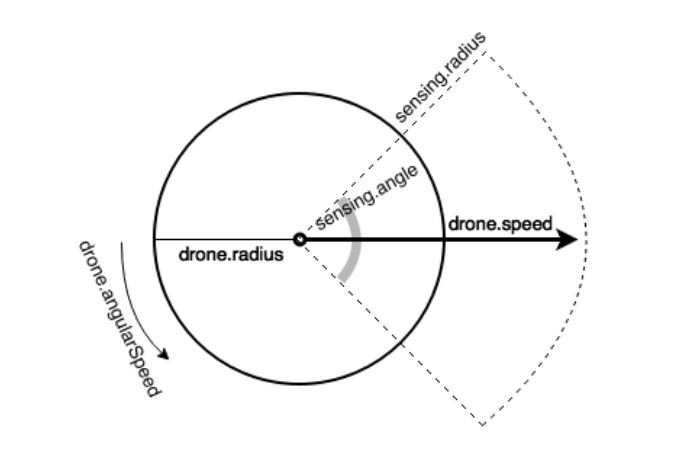
\includegraphics[width=0.4\paperwidth]{img/modello_parametrico_drone.png}}
    \end{center}
    \caption[short]{Modello parametrico del drone.}
    \label{modello_drone}
\end{figure}

La seguente tabella riassume i parametri strutturali che caratterizzano il drone.
\begin{table}[]
    \centering
    \begin{tabular}{|l|l|c|}
    \hline
    \textbf{Parametro}       & \textbf{Definizione}       & \textbf{Unità di misura}   \\ \hline
    drone.radius             & Raggio fisico              & (m)                        \\ \hline
    sensing.radius           & Raggio di sensing          & (m)                        \\ \hline
    sensing.angle            & Angolo di sensing          & (gradi)                    \\ \hline
    drone.cruisingSpeed      & Velocità di crociera       & (m/s)                      \\ \hline
    drone.speedMax           & Velocità massima           & (m/s)                      \\ \hline
    drone.speed              & Velocità corrente          & (m/s)                      \\ \hline
    drone.acceleration       & Accelerazione              & (m/s\textsuperscript{2})   \\ \hline
    drone.deceleration       & Decelerazione              & (m/s\textsuperscript{2})   \\ \hline
    drone.endurance          & Autonomia                  & (minuti)                   \\ \hline
    drone.heading            & Direzione corrente         & (gradi)                    \\ \hline
    drone.accelerationAng    & Accelerazione angolare     & (rad/s\textsuperscript{2}) \\ \hline
    drone.decelerationAng    & Decelerazione angolare     & (rad/s\textsuperscript{2}) \\ \hline
    drone.velocityAngularMax & Velocità angolare massima  & (rad/s\textsuperscript{2}) \\ \hline
    drone.angularSpeed       & Velocità angolare corrente & (rad/s\textsuperscript{2}) \\ \hline
    \end{tabular}
    \caption{Parametri strutturali del drone.}
\end{table}

Ad ogni ciclo di aggiornamento, il drone assume una posizione specifica nello spazio di ricerca, descritta da una coppia di coordinate.
Esso può essere equipaggiato con uno o più sensori e può muoversi sia in modo longitudinale che rotazionale.
Il drone, inoltre, è anche in grado di rilevare i target e di rilasciare impronte di feromone per la comunicazione indiretta con gli altri UAV.

\begin{figure}[H] 
    \captionsetup{justification=centering, margin=2cm, font=footnotesize}
    \begin{center}
    \makebox[\textwidth]{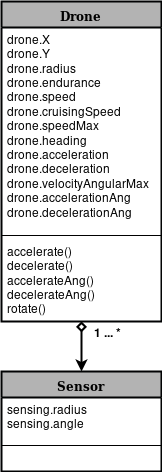
\includegraphics[width=0.2\paperwidth]{img/classe_drone.png}}
    \end{center}
    \caption[short]{Struttura della classe Drone.}
    \label{classe_drone}
\end{figure}

\subsubsection{Progettazione del flocking}

\subsubsection{Progettazione del meccanismo di collision avoidance}

\subsubsection{Progettazione dell'impronta di feromone attrattivo}

\subsection{Algortmi PAPER}